% !TEX TS-program = xelatex
% !TEX encoding = UTF-8 Unicode

\documentclass[a4paper,twoside,12pt]{book}
%\usepackage[utf8]{inputenc}
\usepackage{fontspec}
\usepackage{graphicx}
%\usepackage[russian]{babel}

\setmainfont{Times New Roman}
\setsansfont{Arial}
\setmonofont{Courier New}
\newfontfamily\cyrillicfont[Script=Cyrillic]{Georgia}
\newfontfamily\cyrillicfontsf[Script=Cyrillic]{Arial}
\newfontfamily\cyrillicfonttt[Script=Cyrillic]{Consolas}
\usepackage{polyglossia}
\setdefaultlanguage{russian}

\usepackage{hyperref}
%\hypersetup{pdftex,colorlinks=true,allcolors=blue}
\usepackage{hypcap}
\usepackage{color}
\usepackage{listings}
\usepackage{multirow}

\graphicspath{ {Pics/} }

%% Times New Roman
%\setromanfont[
%BoldFont=timesbd.ttf,
%ItalicFont=timesi.ttf,
%BoldItalicFont=timesbi.ttf,
%]{times.ttf}
%% Arial
%\setsansfont[
%BoldFont=arialbd.ttf,
%ItalicFont=ariali.ttf,
%BoldItalicFont=arialbi.ttf
%]{arial.ttf}
%% Courier New
%\setmonofont[Scale=0.90,
%BoldFont=courbd.ttf,
%ItalicFont=couri.ttf,
%BoldItalicFont=courbi.ttf,
%Color={0019D4}
%]{cour.ttf}

\begin{document}

\author{Алексей Миронов}
\title{Программирование\\
для АБИС "ИРБИС64"\\
в среде .NET Framework}
\date{Июль 2016}

\frontmatter
\maketitle

\lstset{ %
	language=[Sharp]C,                 % выбор языка для подсветки (здесь это С#)
	basicstyle=\ttfamily\small, % размер и начертание шрифта для подсветки кода
	keywordstyle=\color{blue}\textbf,
%	numbers=left,               % где поставить нумерацию строк (слева\справа)
%	numberstyle=\small,          % размер шрифта для номеров строк
%	stepnumber=1,                % размер шага между двумя номерами строк
%	numbersep=7pt,      % как далеко отстоят номера строк от подсвечиваемого кода
%	backgroundcolor=\color{white}, % цвет фона подсветки 
%	% используем \usepackage{color}
%	showspaces=false,        % показывать или нет пробелы специальными отступами
	showstringspaces=false,    % показывать или нет пробелы в строках
	showtabs=false,            % показывать или нет табуляцию в строках
%	frame=single,              % рисовать рамку вокруг кода
	tabsize=2,                % размер табуляции по умолчанию равен 2 пробелам
%	captionpos=t,              % позиция заголовка вверху [t] или внизу [b] 
	breaklines=true,           % автоматически переносить строки (да\нет)
%	breakatwhitespace=false,   % переносить строки только если есть пробел
%	escapeinside={\%*}{*)},     % если нужно добавить комментарии в коде
	stringstyle=\color{red}   % стиль (цвет) строковых литералов
}

\clearpage
\thispagestyle{empty}
	Описаны возможности расширения АБИС "ИРБИС64",
	серверный протокол и фреймворк ManagedIrbis,
	позволяющий создавать приложения произвольной
	сложности на основе "ИРБИС64".
	
	Для автоматизаторов библиотек и программистов,
	создающих решения для "ИРБИС64".

\tableofcontents

\mainmatter
\chapter*{Введение}
\addcontentsline{toc}{chapter}{Введение}
\chaptermark{Введение}

Фреймворк «ManagedIrbis» предназначен для организации программного доступа к ресурсам, находящихся под управлением сервера ИРБИС64, и может использоваться для как для расширения функциональности стандартных АРМ, входящих в поставку АБИС ИРБИС64, так и для создания собственных программных продуктов, совместимых с ИРБИС64.

\section*{Совместимость}

Фреймворк совместим со следующими версиями ИРБИС64:
2004	2005	2006	2007	2008	2009	2010	2011	2012	2013	2014	2015

Совместимость с конкретной версией сервера ИРБИС64 устанавливается по результатам прогона набора стандартных тестов: подключение к серверу, получение служебной информации (версия сервера, количество лицензий и т. д.), чтение записей, форматирование записей, сохранение записей и т. д.

\section*{Инструментарий}

Фреймворк написан на языке C\# в среде Microsoft Visual Studio 2013 для Micorsoft .NET Framework 4.5. Для сборки библиотеки из исходных текстов необходим совместимый инструментарий: Visual Studio 2013 или более новой версии как бесплатной редакции (Express), так и платной (Standard, Profes\-sional и т. д.).

Библиотека должна без модификации успешно собираться средами Mono\-Develop (версия не ниже 4.0) и Sharp\-Develop (версия не ниже 4.4).
Однако всё многообразие альтернативного инструментария не было протестировано авторами (и они не ставили перед собой подобной задачи), и авторы рекомендуют использовать для сборки Visual Studio 2013.

\section*{Системные требования}

Основным системным требованием библиотеки является наличие Microsoft.Net framework 4.5/4.5.1/4.5.2 или совместимой с ним среды исполнения управляемого кода.
Фреймворк должен функционировать в следующем окружении:

\begin{table}[htbp]
	\centering
	\caption{Поддерживаемые окружения}
	\begin{tabular}{ | p{0.4\textwidth} | p{0.4\textwidth} | }
	\hline
	\textbf{Окружение} & 
	\textbf{Функционирование, требования}
	\\
	\hline
	\hline
	Microsoft Windows XP & Не поддерживается \\
	\hline
	Microsoft Windows Vista SP2 & Необходимо установить .Net framework 4.5 \\
	\hline
	Microsoft Windows Server 2003 & Не поддерживается \\
	\hline
	Microsoft Windows 7 SP1 & Необходимо установить .Net framework 4.5 \\
	\hline
	Microsoft Windows Server 2008 SP2/2008 R2 SP1 & Необходимо установить .Net framework 4.5 \\
	\hline
	Microsoft Windows Server 2012/2012 R2 & Предустановлен в операционной системе \\
	\hline
	\end{tabular}
\end{table}

\section*{ManagedIrbis в Интернет}

Исходные коды фреймворка размещены на Git-хостинге github.com по адресу https://github.com/amironov73/arsmagna. Доступ к репозиторию открыт на чтение для всех.
Исполняемые файлы фреймворка опубликованы на сервисе NuGet по адресу

\section*{Лицензия}

Фреймворк распространяется как продукт с открытым исходным кодом. Любой желающий может:

\begin{itemize}
	\item Использовать бинарный релиз библиотеки в своих проектах в неизменном виде – в этом случае требуется лишь указание на авторство библиотеки.
	\item Адаптировать исходный код для собственных нужд и использовать в своих проектах модифицированную версию библиотеки или [модифицированные] фрагменты кода из неё – в этом случае требуется указание на авторство библиотеки и факт модификации её кода.
\end{itemize}

Никаких лицензионных отчислений в вышеперечисленных случаях не требуется. 

\section*{Благодарности}

Авторы выражают благодарность:

\begin{itemize}
	\item \textbf{Ивану Батраку} (СФУ), протестировавшему библиотеку на совместимость со старыми версиями ИРБИС-сервера;
	\item \textbf{Арсению Валентиновичу Шувалову} (Саратовская государственная консерватория им. Л. В. Собинова), выявившему ошибки в библиотеке;
	\item \textbf{Артёму Васильевичу Гончарову} (Научная музыкальная библиотека Санкт-Петер\-бургской Консерватории им. Н. А. Римского-Корсакова), выявившему некоторые досадные ошибки в библиотеке.
\end{itemize}

\section*{Версии и совместимость}

Данное руководство описывает версию 1.3.0.24 библиотеки. Версия библиотеки физически хранится как ресурс VERSION сборки ManagedClient.dll и как статическое свойство Version класса ManagedClient64.

Подробнее о проверке версий см. пункт «Определение версии сервера и клиента».
На данный момент несовместимых версий библиотеки нет, поэтому обновление может осуществляться простым копированием новой сборки поверх старой.
Все будущие несовместимости, если таковые появятся, будут описаны в данном разделе.



\chapter{ИРБИС64-сервер и его окружение}

\begin{description}
	\item[Сервер] это сервер
	\item[Клиент] это клиент
\end{description}

У попа была собака. Он её любил. Она съела кусок мяса. Он её убил. В землю закопал. Надпись написал. У попа была собака. Он её любил. Она съела кусок мяса. Он её убил. В землю закопал. Надпись написал.

У попа была собака. Он её любил. Она съела кусок мяса. Он её убил. В землю закопал. Надпись написал. У попа была собака. Он её любил. Она съела кусок мяса. Он её убил. В землю закопал. Надпись написал. У попа была собака. Он её любил. Она съела кусок мяса. Он её убил. В землю закопал. Надпись написал.

У попа была собака. Он её любил. Она съела кусок мяса. Он её убил. В землю закопал. Надпись написал.

У попа была собака. Он её любил. Она съела кусок мяса. Он её убил. В землю закопал. Надпись написал.

У попа была собака. Он её любил. Она съела кусок мяса. Он её убил. В землю закопал. Надпись написал. У попа была собака. Он её любил. Она съела кусок мяса. Он её убил. В землю закопал. Надпись написал.
\chapter{Протокол ИРБИС64}

У попа была собака. Он её любил. Она съела кусок мяса. Он её убил. В землю закопал. Надпись написал. У попа была собака. Он её любил. Она съела кусок мяса. Он её убил. В землю закопал. Надпись написал.

У попа была собака. Он её любил. Она съела кусок мяса. Он её убил. В землю закопал. Надпись написал. У попа была собака. Он её любил. Она съела кусок мяса. Он её убил. В землю закопал. Надпись написал. У попа была собака. Он её любил. Она съела кусок мяса. Он её убил. В землю закопал. Надпись написал.

У попа была собака. Он её любил. Она съела кусок мяса. Он её убил. В землю закопал. Надпись написал.

У попа была собака. Он её любил. Она съела кусок мяса. Он её убил. В землю закопал. Надпись написал.

У попа была собака. Он её любил. Она съела кусок мяса. Он её убил. В землю закопал. Надпись написал. У попа была собака. Он её любил. Она съела кусок мяса. Он её убил. В землю закопал. Надпись написал.
\chapter{ManagedIrbis. Быстрый старт}

У попа была собака. Он её любил. Она съела кусок мяса. Он её убил. В землю закопал. Надпись написал. У попа была собака. Он её любил. Она съела кусок мяса. Он её убил. В землю закопал. Надпись написал.

У попа была собака. Он её любил. Она съела кусок мяса. Он её убил. В землю закопал. Надпись написал. У попа была собака. Он её любил. Она съела кусок мяса. Он её убил. В землю закопал. Надпись написал. У попа была собака. Он её любил. Она съела кусок мяса. Он её убил. В землю закопал. Надпись написал.

У попа была собака. Он её любил. Она съела кусок мяса. Он её убил. В землю закопал. Надпись написал.

У попа была собака. Он её любил. Она съела кусок мяса. Он её убил. В землю закопал. Надпись написал.

У попа была собака. Он её любил. Она съела кусок мяса. Он её убил. В землю закопал. Надпись написал. У попа была собака. Он её любил. Она съела кусок мяса. Он её убил. В землю закопал. Надпись написал.

\begin{figure}[h]
	\centering
	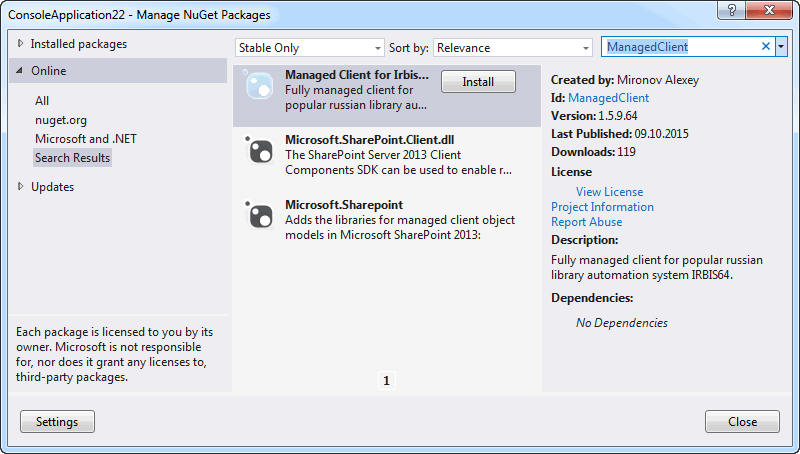
\includegraphics[width=0.7\textwidth]{nuget}
	\caption{Подключение библиотеки через NuGet}
\end{figure}


\begin{lstlisting}
using System;
using System.Linq;

using ManagedIrbis;

class Program
{
  private static void Main()
  {
    try
    {
      using (IrbisConnection connection = new IrbisConnection())
      {
        connection.ParseConnectionString
          (
            "host=127.0.0.1;port=6666;user=1;password=1;"
          );
        connection.Connect();

        int[] foundRecords = connection.Search
          (
            "\"A={0}$\"",
            "А"
          );

        int recordsToShow = Math.Min(foundRecords.Length, 10);

        for (int i = 0; i < recordsToShow; i++)
        {
          int thisMfn = foundRecords[i];

          MarcRecord record = connection.ReadRecord(thisMfn);

          string mainTitle = record
            .Fields
            .GetField("200")
            .GetSubField('a')
            .GetSubFieldText()
            .FirstOrDefault();

          Console.WriteLine
            (
              "MFN={0}, Main title={1}",
              thisMfn,
              mainTitle
            );

          Console.WriteLine
            (
              "BRIEF: {0}",
              client.FormatRecord("@brief", record)
            );

          MarcRecord newRecord = new MarcRecord();
          newRecord.AddField
            (
              "700",
              'a',
              "Управляемый клиент ИРБИС64"
            )
            .AddField
            (
              "200",
              'a', 
              string.Format ("Новая Запись от {0}", DateTime.Now),
              'f',
              "Управляемый клиент"
            );

          connection.WriteRecord
            (
              newRecord, 
              false, 
              true
            );

          Console.WriteLine(new string('-', 60));
        }
      }
    }
    catch (Exception ex)
    {
      Console.WriteLine(ex);
    }
  }
}\end{lstlisting}

\chapter{Описание классов}

\section{Класс ManagedIrbis}

ManagedIrbis – «рабочая лошадка». Этот класс осуществляет связь с сервером, всю необходимую «перепаковку» данных и прочее и прочее. Собственно, это и есть управляемый клиент ИРБИС64.

Экземпляр клиента создаётся конструктором по умолчанию:
\begin{lstlisting}
IrbisConnection client = new IrbisConnection ();
\end{lstlisting}

\subsection{Подключение к серверу}

Параметры подключения к серверу определяются следующими свойствами:

\begin{lstlisting}
public string Host { get; set; }
public int Port { get; set; }
public string Username { get; set; }
public string Password { get; set; }
public string Database { get; set; }
public IrbisWorkstation Workstation { get; set; }
\end{lstlisting}

Обратите внимание, что адрес сервера задаётся строкой, так что может принимать как значения вроде "192.168.1.1", так и "irbis.yourlib.com". 
Если какой-либо вышеперечисленных из параметров подключения не задан явно, используется значение по умолчанию. По умолчанию, клиент готов к работе с локально установленной демо-версией ИРБИС64. :) 
За подключение и отключение отвечают два метода: 
\begin{lstlisting}
void Connect ();
public void Disconnect ();
\end{lstlisting}
При возникновении ошибки при подключении метод Connect выбросит исключение. 

После успешного установления соединения повторные вызовы Connect не выполняют никаких действий. Аналогично после успешного отключения повторные вызовы Disconnect не выполняют никаких действий. 

Проверить, подключены ли мы в данный момент к серверу, можно с помощью свойства Connected:
\begin{lstlisting}
public bool Connected { get; }
\end{lstlisting} 
Вместо индивидуального задания каждого из параметров Host, Port, Username, Password и Database, можно использовать метод ParseConnectionString: 
\begin{lstlisting}
public void ParseConnectionString ( string connectionString );
\end{lstlisting}
Рекомендуется заключать всю работу с клиентом в контекстные скобки using языка C\# для корректного освобождения ресурсов при возникновении нештатных ситуаций. 

Метод GetMaxMfn возвращает максимальный номер MFN в базе данных:
\begin{lstlisting}
public int GetMaxMfn ();
\end{lstlisting}
Метод IsDatabaseLocked, определяет, не установлена ли в данный момент монопольная блокировка на базу данных: 
\begin{lstlisting}
public bool IsDatabaseLocked ( string databaseName ); // Необходимо указать имя базы данных
\end{lstlisting}
Пример подключения к серверу: 
\begin{lstlisting}
using (var client = new IrbisConnection ())
{
	string connectionString = System.Configuration.AppSettings["connection-string"];
	client.ParseConnectionString ( connectionString );
	client.Connect ();

	Console.WriteLine ( "Записей в базе: {0}", client.GetMaxMfn() - 1 );
}
\end{lstlisting}

\subsection{Работа с базой данных}

Имя текущей базы данных (каталога), с которой работает клиент, хранится в поле Database:
\begin{lstlisting}
public string Database { get; set; }
\end{lstlisting}
Кроме того, имеются два полезных метода:
\begin{lstlisting}
/// Временно устанавливает новое имя текущей базы данных.
/// Запоминает, к какой базе был подключен
/// клиент на момент смены.
/// Возвращает имя предыдущей текущей базы данных.
public string PushDatabase(string newDatabase);

/// Восстанавливает подключение к предыдущей базе данных,
/// сменённой методом PushDatabase().
/// Возвращает имя базы данных, к которой был подключен 
/// клиент на момент восстановления состояния.
public string PopDatabase()
\end{lstlisting}
Оба метода работают по принципу стека: предыдущие базы данных запоминаются в стеке и постепенно возвращаются по мере вызова метода PopDatabase(). Пример:
\begin{lstlisting}
// Мы работали с базой IBIS, 
// но решили временно подключиться к RDR
client.PushDatabase ("RDR"); // IBIS запоминается в стеке
IrbisRecord reader = client.SearchReadOneRecord ("I=1234");

// Теперь временно подключаемся к RQST
client.PushDatabase ("RQST"); // RDR также запоминается в стеке
IrbisRecord request = new IrbisRecord ();
...
client.WriteRecord (request, false, true); // Запись пойдёт в RQST

...
// Возвращаемся к базе RDR
client.PopDatabase ();
client.WriteRecord (reader, false, true); // Запись пойдёт в RDR

...
// Возвращаемся к исходной базе IBIS
client.PopDatabase ();
Рекомендую временные переключения между базами оформлять в блоке try-finally: 
client.PushDatabase ("CMPL");
try
{
   // Какие-то манипуляции с базой
}
finally
{
  // Гарантированно возвращаемся в правильный контекст
  // работы с базой данных
  client.PopDatabase();
}
\end{lstlisting}

\subsection{Многопоточность и состояние занятости}

Клиент написан в наивном однопоточном стиле, поэтому не поддерживает одновременное выполнение команд из разных потоков. Во время обращения к серверу устанавливается флаг
\begin{lstlisting}
public bool Busy { get; }
\end{lstlisting}
\subsection{Подтверждение подключения}

Библиотека самостоятельно не посылает на сервер подтверждений того, что клиент всё ещё подключен. Этим должно заниматься приложение, например, по таймеру. 

Подтверждение посылается серверу методом NoOp:
\begin{lstlisting}
public void NoOp ();
\end{lstlisting}
\subsection{Чтение/сохранение записей}

Методы для чтения и сохранения записей (класс MarcRecord будет рассмотрен позже, пока воспринимайте его как «чёрный ящик»): 
\begin{lstlisting}
public IrbisRecord ReadRecord ( int mfn ); // Чтение одной записи по её MFN
public IrbisRecord[] ReadRecords ( IEnumerable<int> mfns ); // Чтение массива записей с указанными MFN
public void WriteRecord ( IrbisRecord record, bool needLock, bool ifUpdate ); // Сохранение одной записи
				// needLock – оставить запись заблокированной
				// ifUpdate – обновить инвертированный файл (поисковый индекс)
public void WriteRecords ( IrbisRecord[] records, bool ifUpdate ); // Сохранение массива записей
				// ifUpdate – обновить инвертированный файл (поисковый индекс)
\end{lstlisting}
Запись «помнит» свой MFN, поэтому заботиться о том, чтобы модифицированная запись встала на нужное место, не нужно. Вновь созданная запись имеет MFN=0, поэтому будет помещена в конец мастер-файла. После первого сохранения её MFN автоматически сменится на реально используемый.

Кроме того, фреймворк автоматически отслеживает изменение версии записи, а также модификации, вносимые сервером при сохранении (отработка autoin.gbl).

\subsection{Поиск записей}

Метод для поиска записей: 
\begin{lstlisting}
public int[] Search ( string format, params object[] args ); // возвращает массив MFN записей, 
// удовлетворяющих запросу
\end{lstlisting}
Если ни одной записи не найдено, возвращается массив из 0 элементов. 

Пример вызова:
\begin{lstlisting}
string authorName = "Иванов"; // фамилия автора книги
int[] mfns = client.Search ( "\"A={0}$\"", authorName ); // поиск по соответствующему префиксу
// обратите внимание на знак доллара, означающий усечение справа
// и на кавычки, обрамляющие запрос
Поиск с одновременным чтением: 
public IrbisRecord[] SearchRead ( string format, params object[] args ); // Возвращает записи,
			// удовлетворяющие запросу. По факту совмещает методы Search и ReadRecord

Если ни одной записи не найдено, возвращается массив из 0 элементов. 
Пример вызова: 
foreach ( var record in client.SearchRead ( "J=CHI" ) ) // ищем книги на китайском языке
{
	// Обрабатываем записи по одной
	Console.WriteLine ( "Найдено: {0}", record );
}
\end{lstlisting}

\subsection{Форматирование записей}
 
Во всех нижеперечисленных методах строка format может принимать одно из трёх значений:
\begin{itemize}
	\item Собственно формат на языке ИРБИС, например "v200\^a, ' : ', v200\^e";
	\item Ссылку на серверный pft-файл, начинающуюся с символа "@" (без расширения pft), например: "@brief";
	\item Ссылку на оптимизированный формат (какой формат использовать, определит сам сервер, основываясь на механизме оптимизации форматов просмотра), состоящую из единственного символа "@".
\end{itemize}

Методы для форматирования записей: 
\begin{lstlisting}
public string FormatRecord
	(
		string format,
		int mfn
	);
	
public string FormatRecord
	(
		string format,
		MarcRecord record
	);
	
public string[] FormatRecords
	(
		string format,
		int[] mfns
	);
	
public string[] SearchFormat
	(
		string expression,
		string format
	);
\end{lstlisting}
Пример вызова:
\begin{lstlisting}
foreach ( var description in connection.SearchFormat ( "G=2000", "@brief" ) )
{
	Console.WriteLine ( description );
}
\end{lstlisting}
\section{Классы MarcRecord, RecordField и SubField}

Каждый экземпляр класса IrbisRecord соответствует одной записи в базе данных ИРБИС. Он содержит следующие элементы:
\begin{lstlisting}
public string Database { get; } // Имя базы данных, из которой считана запись. 
			// Для вновь созданных записей содержит null
public int Mfn { get; } // Номер записи в мастер-файле.
			// Для вновь созданных записей равен 0
public RecordStatus Status { get; } // Статус записи – логически удалена, 
			// физически удалена и т. д.
public int Version { get; } // Версия записи. 
			// Устанавливается сервером автоматически
public bool Deleted { get; set; } // Признак удалённой записи
			// (чтобы не возиться лишний раз с полем Status)
public List<RecordField> Fields { get; } // Список полей записи
\end{lstlisting}
Запись хранит поля в списке Fields. Каждое поле соответствует экземпляру класса RecordField, который содержит следующие элементы:
\begin{lstlisting}
public string Tag { get; set;} // Метка поля
public string Text { get; set; } // Значение поля
public string List<SubField> SubFields { get; } // Список подполей
\end{lstlisting}
Поле хранит подполя в списке SubFields. Каждое подполе соответствует экземпляру класса SubField, который содержит следующие элементы:
\begin{lstlisting}
public char Code { get; set; } // Код подполя
public string Text { get; set; } // Значение подполя
\end{lstlisting}
\subsection{Манипуляции с записями}

Получаем значение первого повторения поля (Field Match):
\begin{lstlisting}
string language = record.FM ( "101" ); // Язык основного текста документа
\end{lstlisting}
Если такого поля нет, возвращается null.

Получаем массив всех повторений данного поля (Field Match All):
\begin{lstlisting}
string[] keywords = record.FMA ( "610" ); // Все ключевые слова
\end{lstlisting}
Если таких полей нет, возвращается массив из 0 элементов. 

Получаем значение первого повторения подполя:
\begin{lstlisting}
string title = record.FM ( "200", 'a' ); // Основное заглавие
\end{lstlisting}
Если такого поля/подполя нет, возвращается null.

Получаем массив всех повторений данного подполя:
\begin{lstlisting}
string[] subjects = record.FMA ( "606", 'a' ); // Все предметные заголовки
\end{lstlisting}
Если таких полей/подполей нет, возвращается массив из 0 элементов. 

Выясняем, есть ли в записи хоть одно поле из перечисленных: 
\begin{lstlisting}
if (record.HaveField ( "606", "607" ))
{
	Console.WriteLine ( "Есть рубрики!");
}
\end{lstlisting}
Проверяем отсутствие всех перечисленных полей:
\begin{lstlisting}
if (record.HaveNotField ( "700", "701", "702" ))
{
	Console.WriteLine ( "Нет точек доступа на авторов!" );
}
\end{lstlisting}
Удаляем все повторения указанного поля (если поля нет, ничего не происходит):
\begin{lstlisting}
record.RemoveField ( "331" ); // Удалили аннотацию
\end{lstlisting}
Добавляем поле с текстом:
\begin{lstlisting}
record.AddField ( "300", "Авторы указаны на корешке" );
\end{lstlisting}
Добавляем поле с подполями:
\begin{lstlisting}
record.AddField ( "200", 'a', "Заглавие",
	'e', "подзаголовочные сведения",
	'f', "сведения об ответственности" );
\end{lstlisting}
Устанавливаем первое повторение поля с текстом (если поля с такой меткой нет, оно будет создано):
\begin{lstlisting}
record.SetField ( "102", "RU" ); // Код страны
\end{lstlisting}
Обратите внимание, что вызовы AddField, SetField и RemoveField могут «цепляться» друг за друга для повышения читабельности программы:
\begin{lstlisting}
record.RemoveField ( "331" )
	.SetField ( "102", "RU" )
	.AddField ( "300", "Авторы указаны на корешке" );
\end{lstlisting}
Конечно же, запись и все её поля/подполя могут быть созданы «с нуля» с помощью соответствующих конструкторов, после чего запись можно сохранить:
\begin{lstlisting}
var record = new IrbisRecord (); // Создали запись

// Создаём поле 900 и подполя в нём
var field900 = new RecordField ( "900" ); // Коды: тип, вид, характер документа
var sub900b = new SubField ( 'b', "05" ); // Однотомное издание
var sub900t = new SubField ( 't', "a" ); // Текстовый материал
field900.SubFields.Add ( sub900b ); // Добавили подполя в поле
field900.SubFields.Add ( sub900t );
record.Fields.Add ( field900 ); // Добавили поле в запись

var field102 = new RecordField ( "102" ); // Страна
field102.Text = "RU"; // Россия
record.Fields.Add ( field102 );

var field101 = new RecordField ("101"); // Язык основного текста
field101.Text = "rus"; // Русский язык
record.Fields.Add ( field101 );

. . .

// Сохраняем запись, блокировка записи нам не нужна, 
// зато нужно обновление поискового индекса
client.WriteRecord ( record, false, true );
\end{lstlisting}

\subsection{Последовательный поиск}

В простейшем случае этот поиск состоит из указания двух выражений: 1) обычное поисковое выражение, отбирающее записи по словарю, 2) булево выражение, которое будет применено к каждой найденной записи. 

Пример такого поиска: сначала мы отбираем все книги с фамилией автора "Пушкин", а затем проверяем, не содержит ли поле 200 буквосочетания "сказк": 
\begin{lstlisting}
// Выполняем последовательный поиск
int[] found = Client.SequentialSearch
    (
        "\"A=Пушкин$\"", // отбор по словарю
        "v200:'сказк'"   // булево выражение
    );

// Выводим найденные записи на консоль
foreach (int mfn in found)
{
    string description = Client.FormatRecord
        (
            "@brief",
            mfn
        );
    Console.WriteLine(description);
}
\end{lstlisting}
На экран будет выведено что-то вроде: 
\begin{verbatim}
Пушкин, Александр Сергеевич. Сказка о царе Салтане, о сыне его славном и могучем богатыре князе Гвидоне Салтановиче и о прекрасной царевне Лебеди / А.С. Пушкин ; Послесл. М. Сокольникова; Ил. А.М. Куркина (Палех), 1972. - 39 c. 

Пушкин, Александр Сергеевич. Сказки / А.С. Пушкин; Ил. А. Кокорина, 1976. - 72 с. 

Пушкин, Александр Сергеевич. Собрание сочинений : В 10 т. Т.3. : Поэмы. Сказки, 1982. - 671 с. 

Пушкин, Александр Сергеевич. Сказка о царе Салтане,о сыне его славном и могучем богатыре князе Гвидоне Салтановиче и о прекрасной царевне Лебеди / А.С. Пушкин, 1971. - 94 с. 

Пушкин, Александр Сергеевич. Сочинения : в 2 т. Т. 1 : Стихотворения, поэмы, сказки, 1982. - 365 с. 
\end{verbatim}

Есть вариант этого же метода, предоставляющий больший контроль: 
\begin{lstlisting}
Client.SequentialSearch
(
"\"A=Пушкин$\"",
100,   // запрашиваемое количество записей
1,     // номер первой записи (смещение)
10000, // минимальный MFN
20000, // максимальный MFN
"v200:'сказк'"        
);
\end{lstlisting}
Если вместо "\"A=Пушкин\$\"" передать null, то будет выполнен последовательный поиск по всей базе данных, что, скорее всего, создаст большую нагрузку на сервер. 

Подробнее см. документацию на протокол ИРБИС": http://sntnarciss.ru/irbis/spravka/wtcp007007020.htm.
\chapter*{Библиотека AM.Core}
\addcontentsline{toc}{chapter}{Библиотека AM.Core}

\backmatter
% bibliography, glossary and index would go here.

\listoffigures
\addcontentsline{toc}{chapter}{Список иллюстраций}
\listoftables
\addcontentsline{toc}{chapter}{Список таблиц}

\end{document}